\section{The gestures}
As mention in the user stories for the application, all of the application's functionality should be accessible by using gestures. The user should thus
be able to do every task only by using gestures (except the "look around story", which only be done by rotating the HMD). To support this a gesture scheme of seven (or eight depending
on perspective) individual gestures were created. 
These are individually described below on a functional level and will be covered in more technical detail during the next chapter. 
Both the left- and right hand should be able to execute all these gestures independently, so scenarios where both hands do the same gestures, or different gestures, should
work.
 
\subsection{The pinch gesture}
The pinch gesture will cover the "rotate user story", specified in the previous section, and thus enable the user to rotate the camera by the Y and Z axis. 
The pinch gesture is accomplished by squeezing the tip of the thumb and index fingers together while, preferably, keeping the rest of the fingers erect and the palm facing 
somewhere between the table top and the displays (see \ref{fig:gestures1} for an illustration). Once this gesture is done by the user, 
the system should indicate that the gesture was recognized as a pinch gesture.
Once the system has recognized the pinch gesture it sets the x, y and z coordinates where the gesture was detected as an origin point and starts rotating the 
camera with the offset value of this origin point. This means that when the user does a pinch gesture without moving the hand, the pinch gesture should be detected and be
"active", but the camera should not be moved. If the user then moves his or her hand to the right, while still keeping the pinch gesture, the camera should start rotating 
to the right also. If the user moves his or her hand further to the right the camera should start rotate at a faster rate than previously.  
The primary idea behind this origin-offset scheme, which also are used in other gestures, is to prevent user fatigue by allowing the user to execute
the gesture in the position that feels most comfortable, as long as this position is captured by the vision-based gesture recognition system. 
In addition this scheme also prevents the user from having to move his or her hands as much as some other schemes would (e.g.~dragging motions).  

\begin{figure}%[h!] %[H]
	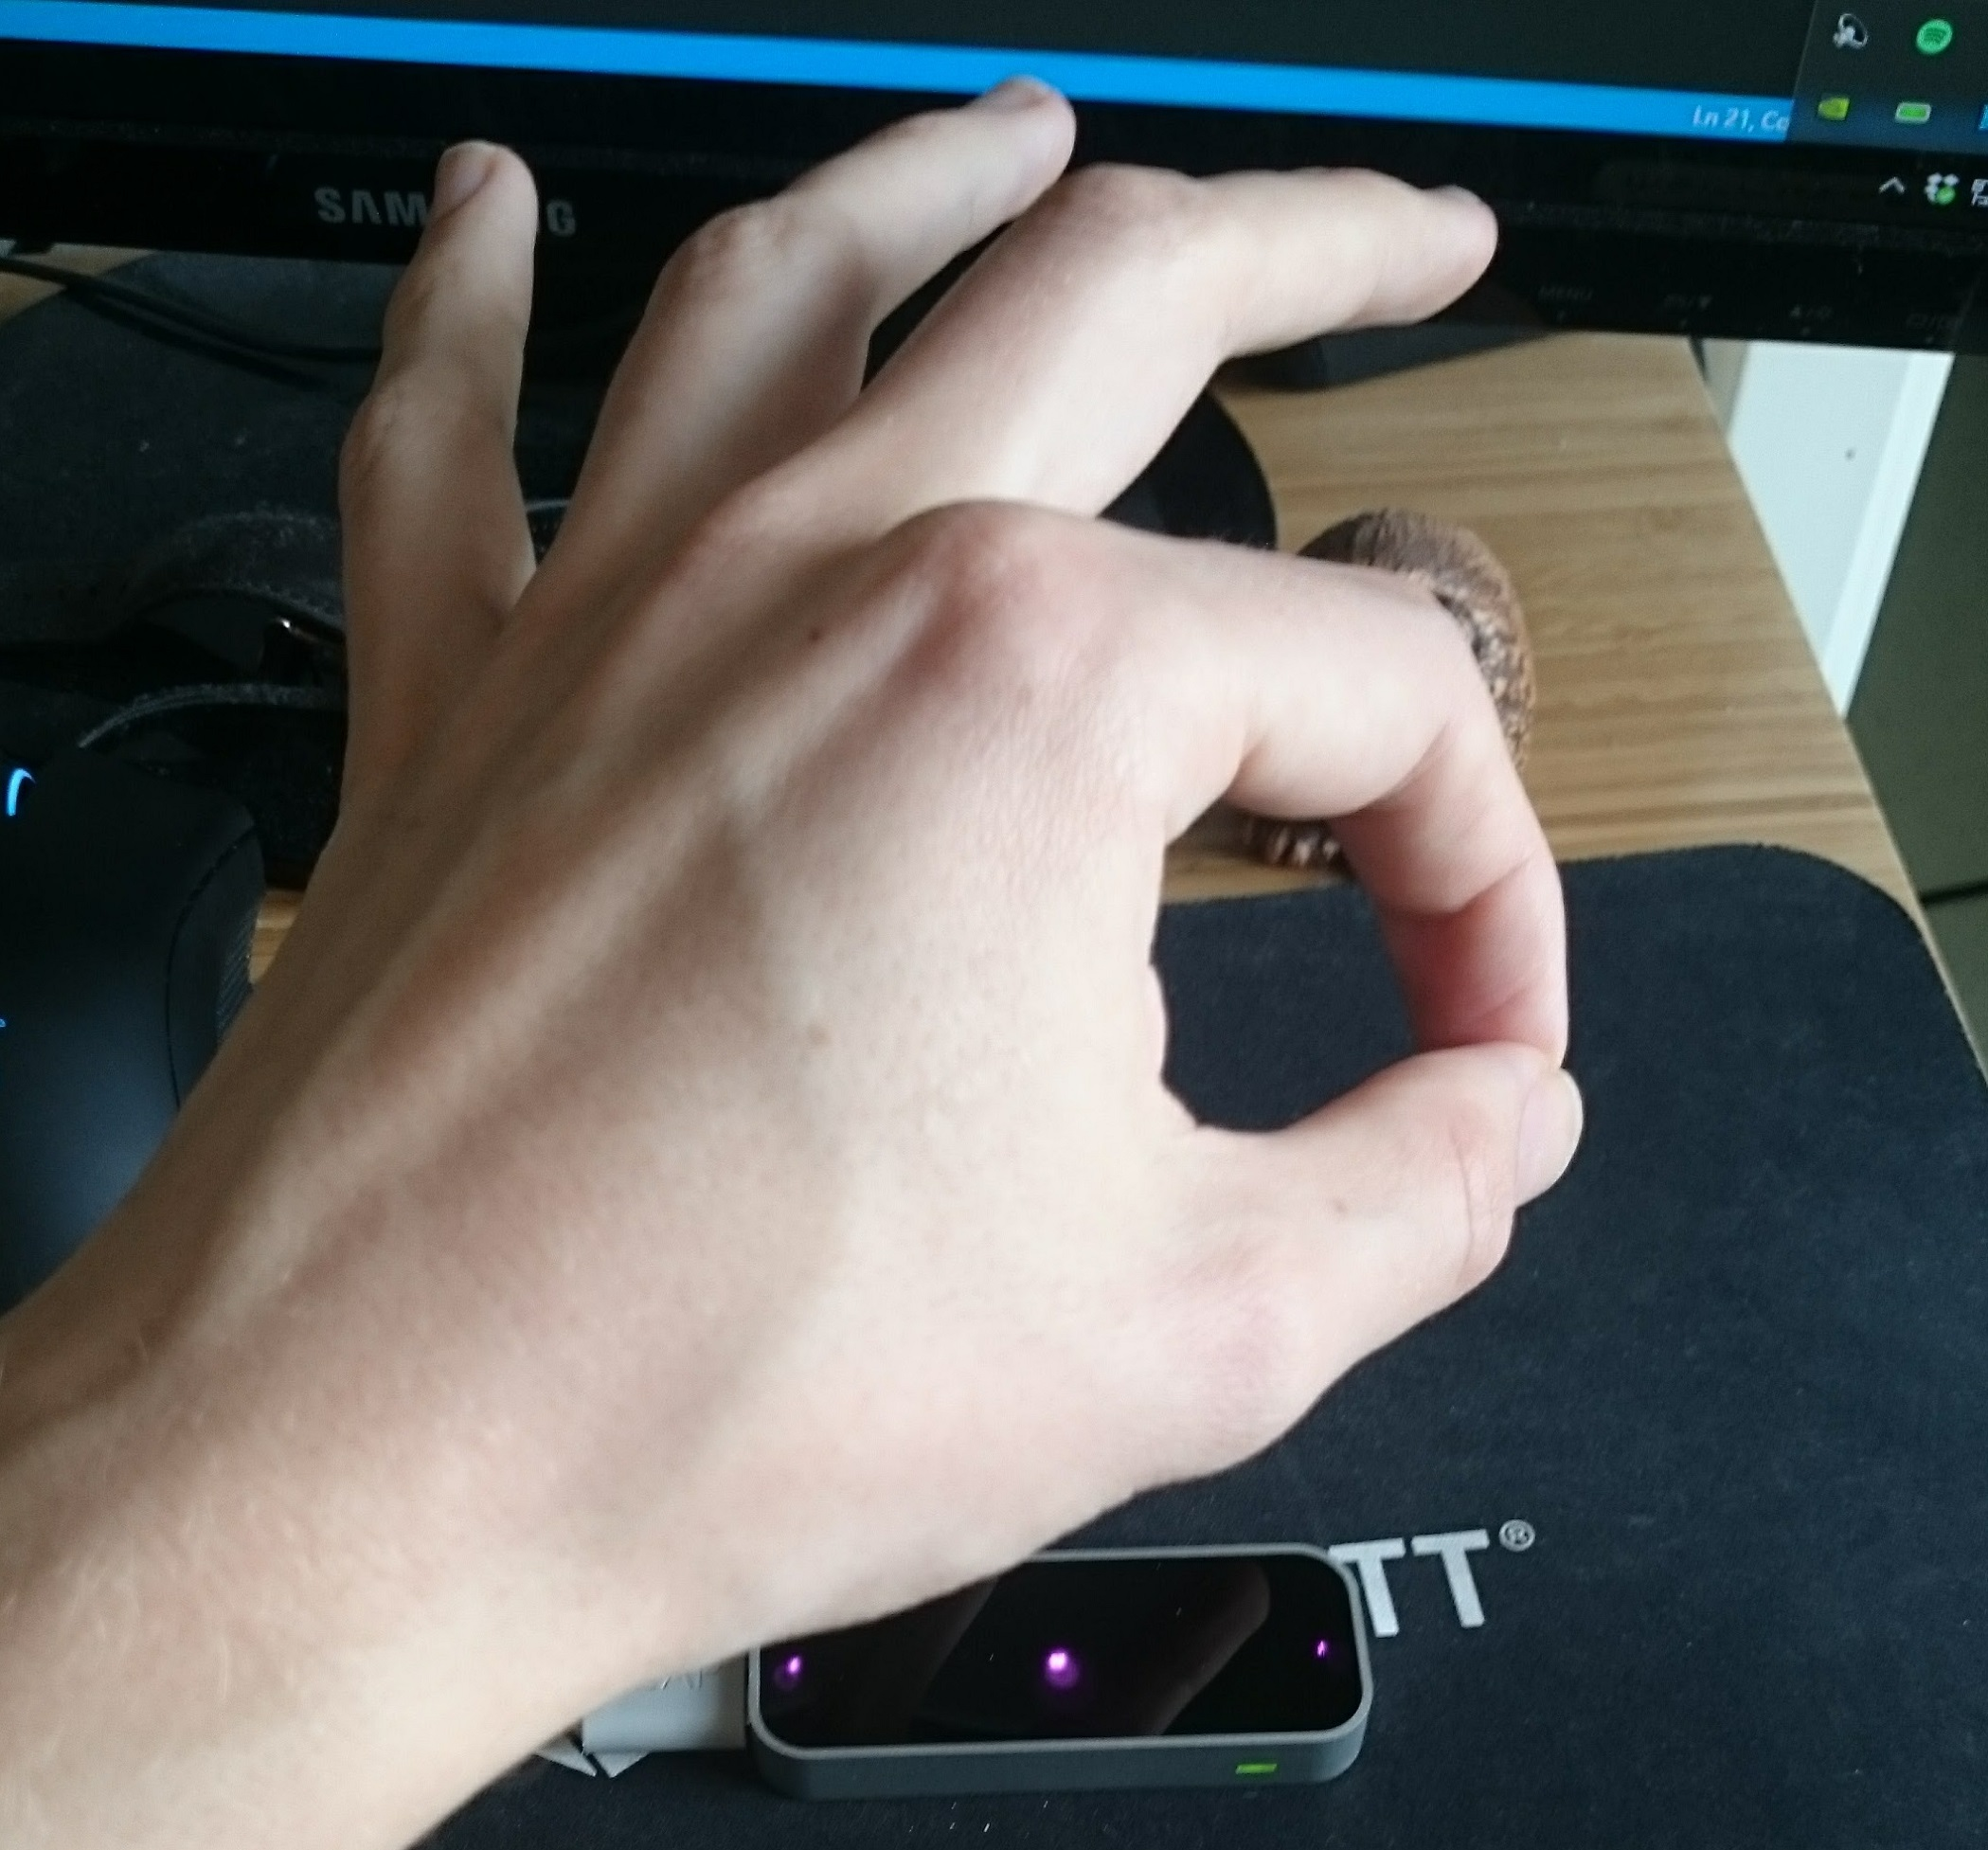
\includegraphics[width=0.5\linewidth]{pictures/gestures/pinch.jpg}
    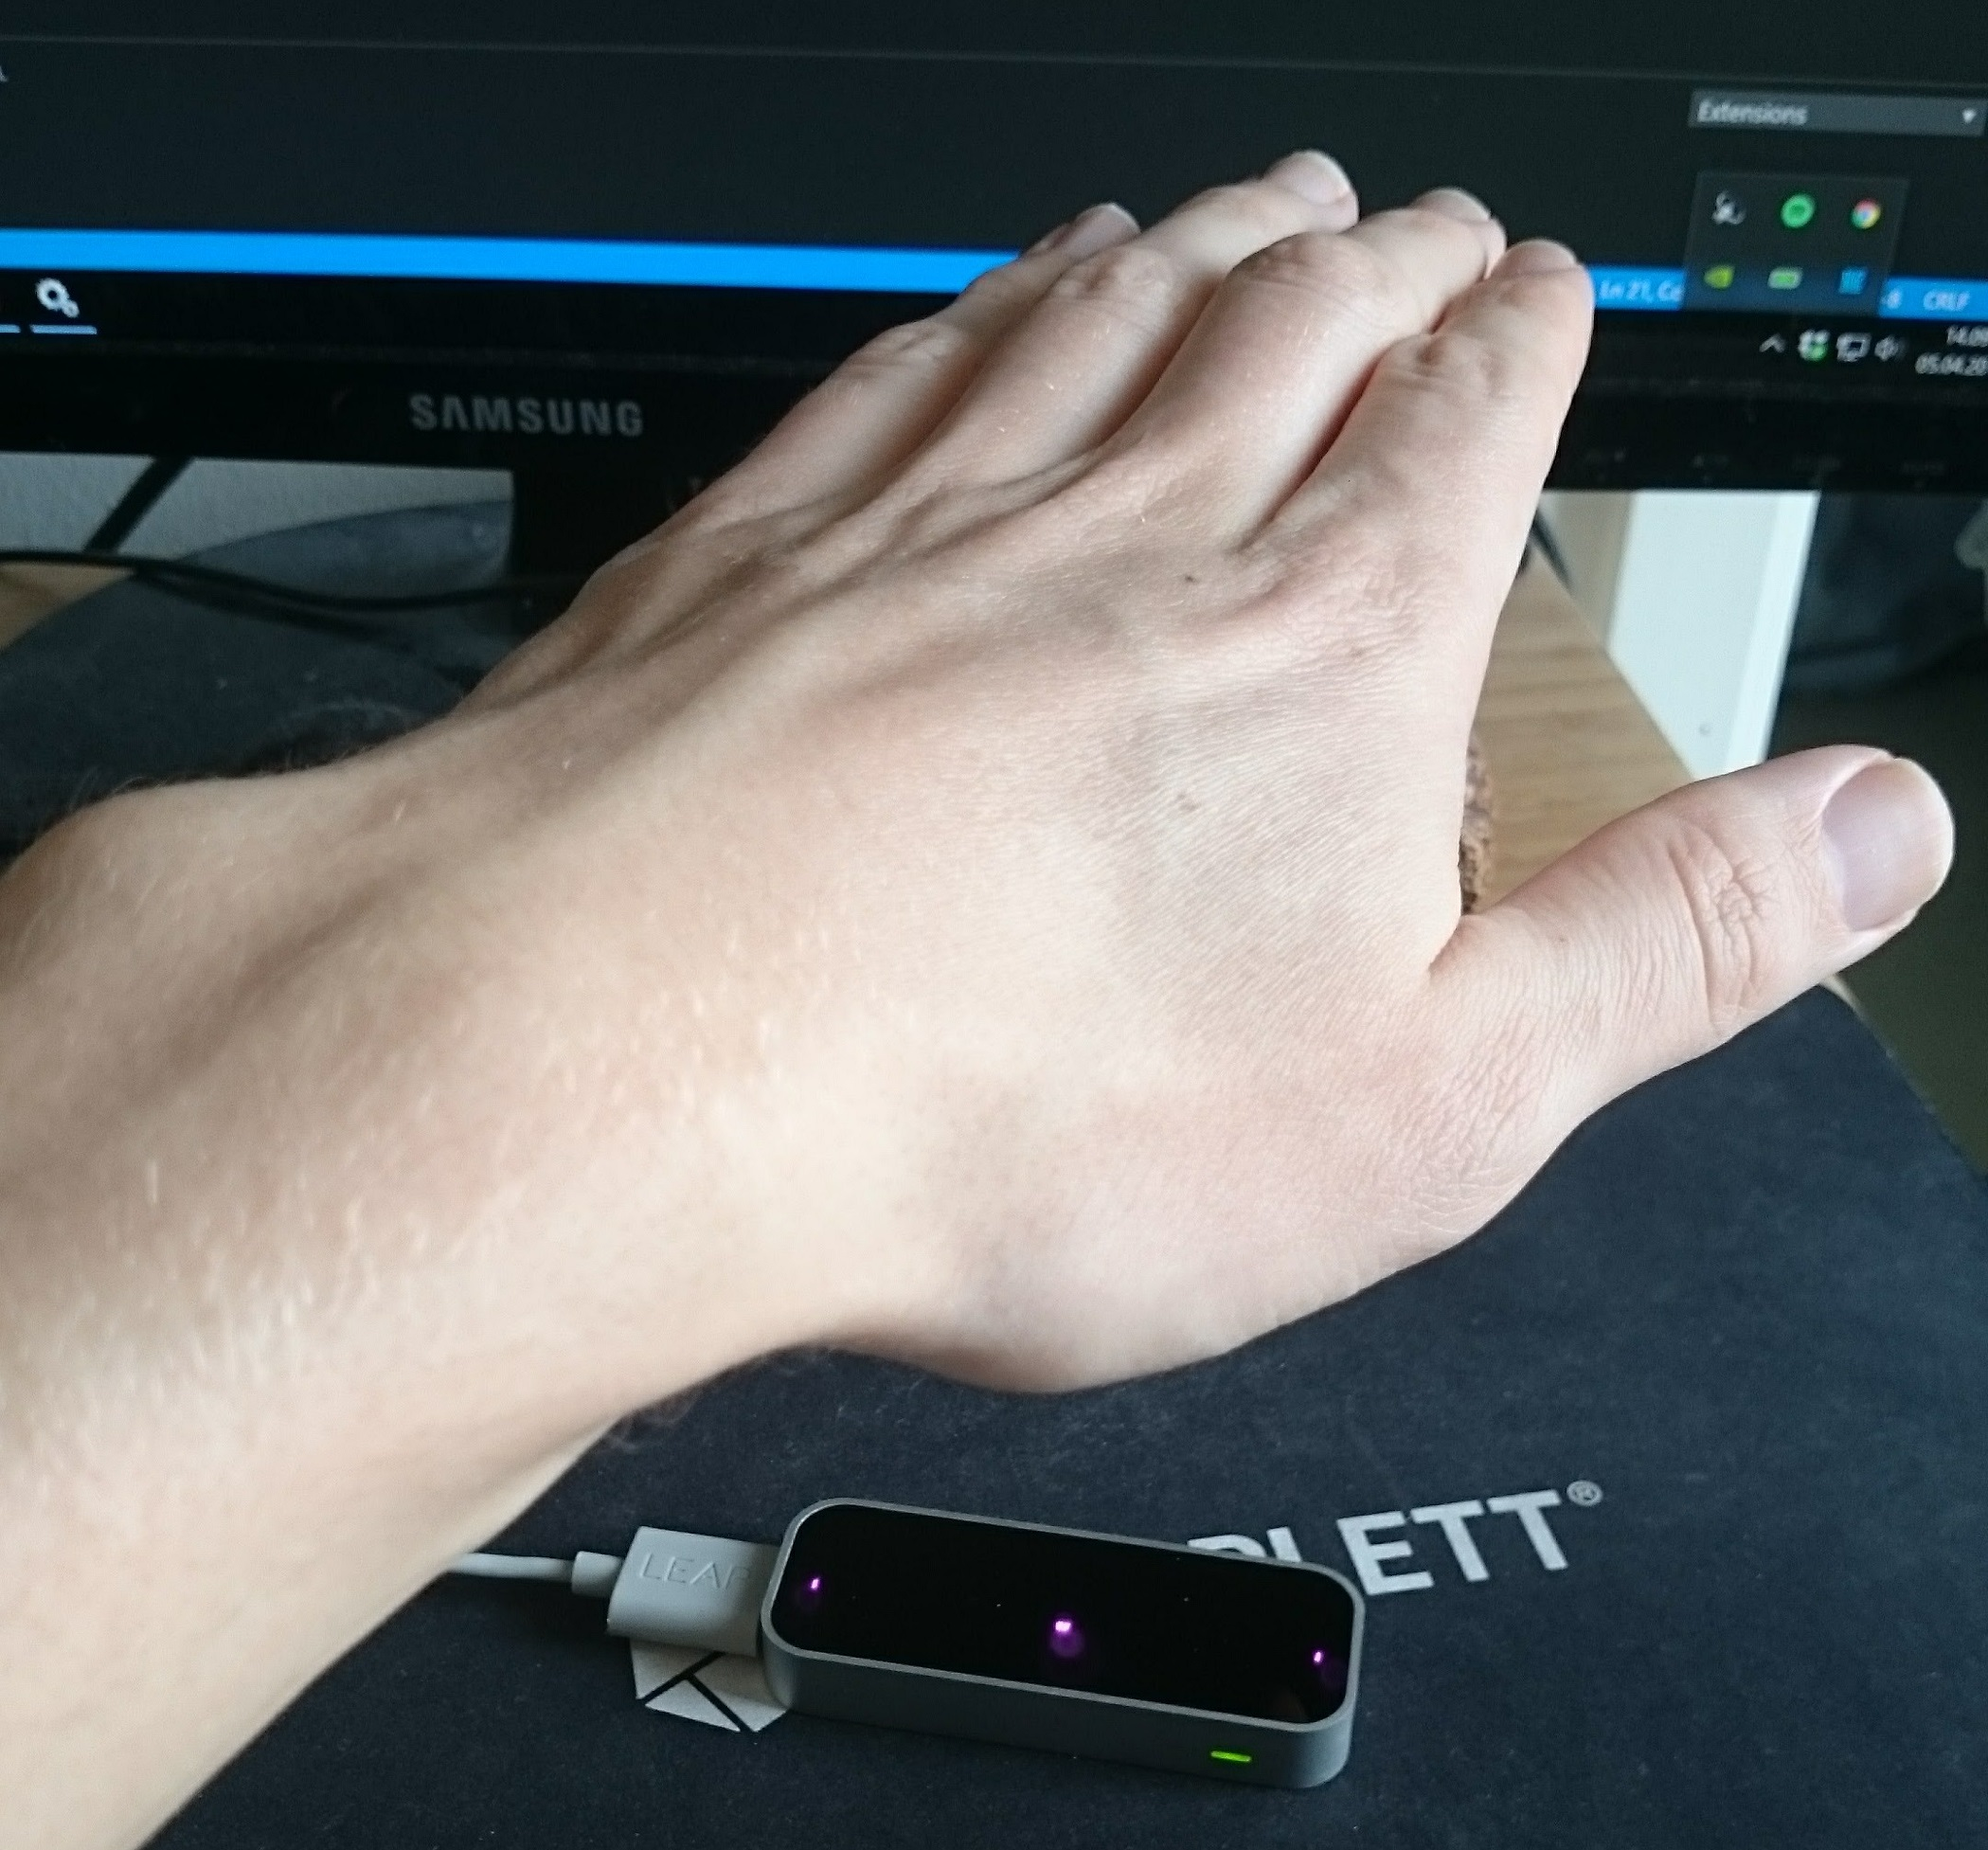
\includegraphics[width=0.5\linewidth]{pictures/gestures/palmdown.jpg}
	\caption[The pinch and palm-down gestures]{The pinch gesture (left) is used to rotate the camera along the y- and z-axis. 
             The palm-down gesture (right) is used to move the user up and down along the y-axis.}
	\label{fig:gestures1}
\end{figure} 

\subsection{The palm-down gesture}
The palm-down gesture, alternatively called the Y-gesture, fulfills the up-and-down functionality specified in the "move-user story", and enables the user to 
move the player model along the y-axis, relative to its orientation. The palm-down gesture is accomplished simply by having all fingers extended, with all of them pointing in
the direction of the display with the palm facing downwards towards the table top (see \ref{fig:gestures1} for an illustration). This gesture, along with the rest of the 
"movement gestures", uses the same origin-offset scheme as the pinch gesture, but the offset is in this gesture only measured on the y-axis, so moving the hand to the 
right, as mention in the pinch gesture section, will cause no movement when the palm-down gesture is the active gesture. 
Instead the user can move his or her hands up and down on the y-axis, so the distance to the table top varies.  

\subsection{The palm-side gesture}
The palm-side gesture, alternatively called the X-gesture, fulfills the left-and-right functionality specified in the "move-user story", and enables the user to 
move the player model along the x-axis, relative to its orientation. The palm-side gesture is accomplished simply by having all fingers extended, with all of them pointing in
the direction of the display with the palm perpendicular (i.e~at a 90° or 270° angle) to the table top (see \ref{fig:gestures1} for an illustration). 
As one of the movement gesture, this gesture also uses the origin-offset scheme, but only with the x-axis monitored.

\subsection{The fist gesture}
The fist gesture, alternatively called the Z-gesture, fulfills the forward-and-backwards functionality specified in the "move-user story", and enables the user to 
move the player model along the z-axis, relative to its orientation. The fist gesture gesture is accomplished by forming a fist (i.e with no fingers extended)
and is used by extending and retracting the fist. 

\subsection{The combined-movement gesture}
The combined-movement gesture, alternatively called the XYZ-gesture, is a special gesture that's only enabled if the "use combined gesture" option is selected in the menu.
When this gesture is enable the other movement gestures, i.e the palm-down-, the palm-side- and the fist gesture, are disabled. If the "use combined gesture" is disabled, 
by clicking "distinguish movement gestures" in the menu, the other movement gestures are once again enabled. This gesture is done in the same manner as the palm-down gesture, 
i.e by having all fingers extended, with all of them pointing in the direction of the display with the palm facing downwards towards the table top.
However, instead of now only being responsible for navigation along the y-axis, i.e up and down, this same gesture is now responsible for movement along the x-, y- and z-axis.
This gesture also used the origin-offset scheme, but now all the three dimensions are monitored. 

\subsection{The point gesture}
The point gesture is used to annotate a point or edit a point annotation, and is used by having the index finger extended and "pointing" at the display while the 
rest of the fingers are non-extended. When the user does the point gesture, a raycast (a kind of invisible beam) should be fired from the 
player model towards where the play model is facing. 

\subsection{The double-point gesture}